%!TEX root = ../main.tex

\section{Исследование обобщения модели}

\begin{frame}{Постановка задачи}
Исследуем распределение фазового поля вокруг проводников ($\phi = 0$) различного вида. Рассмотрим
следующие краевые задачи:
\begin{enumerate}
	\item $\Omega = [0, +\infty)_x \times I_y \times I_z, \; \phi|_{x = 0} = 0, \; \phi \to 1$ при
	$r = x \to +\infty$ -- плоский случай;
	\item $\Omega = \mathbb{R}_x \times \mathbb{R}_y \times I_z, \; \phi|_{x, y = 0} = 0, \;
	\phi \to 1$ при $r = \sqrt{x^2 + y^2} \to +\infty$ -- \\ цилиндрический случай;
	\item $\Omega = \mathbb{R}_x \times \mathbb{R}_y \times \mathbb{R}_z, \;
	\phi|_{x, y, z = 0} = 0, \; \phi \to 1$ при $r = \sqrt{x^2 + y^2 + z^2} \to +\infty$ -- \\
	сферический случай.
\end{enumerate}
Ищем стационарное решение $\phi = \phi(r)$.
\end{frame}


\begin{frame}{Суть проблемы}
\begin{columns}
\column{0.5\textwidth}
\centering
Плоский случай
\column{0.5\textwidth}
\centering
Цилиндрический случай
\end{columns}
\vspace{0.5cm}
\begin{columns}
\column{0.49\textwidth}
Задача Коши:
\vspace{-0.3cm}
$$\phi(0) = 0; \qquad \cfrac{\partial \phi}{\partial x} = \cfrac{2}{l} \sqrt{1 - f(\phi)}$$
\begin{figure}
	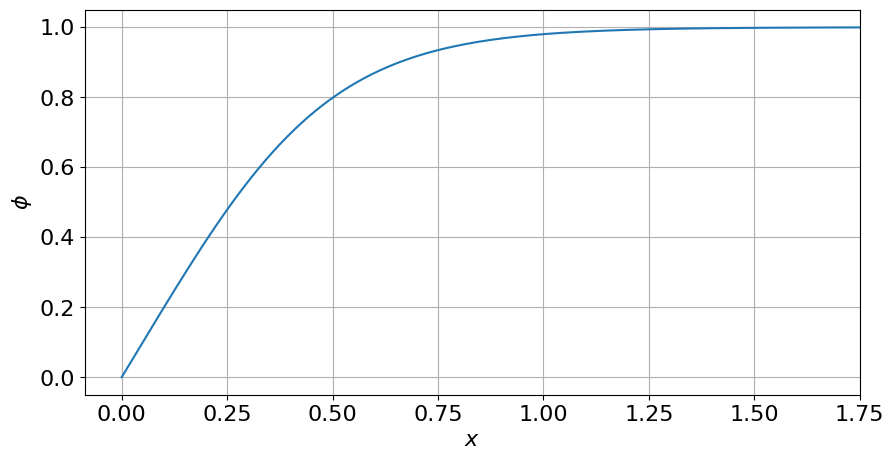
\includegraphics[width=\textwidth]{../figures/result_volumes.png}
\end{figure}
\column{0.01\textwidth}
\rule{0.4pt}{0.7\textheight}
\column{0.49\textwidth}
\centering
Задача поставлена некорректно \\ и решения не имеет \cite{zipunova_higher_codimension}
\end{columns}
\end{frame}


\begin{frame}{Обобщение модели}
\begin{block}{Обобщение модели, предложенное в работе \cite{zipunova_higher_codimension}}
\begin{itemize}
	\item Уравнение электрического потенциала $\Phi$:
	$$\Div(\epsilon[\phi] \nabla \Phi) = 0$$
	\item Уравнение фазового поля $\phi$:
	$$\cfrac{1}{m} \cfrac{\partial \phi}{\partial t} =
    \cfrac{1}{2} \epsilon'(\phi) (\nabla \Phi, \nabla \Phi) +
    \cfrac{\Gamma}{l^2} f'(\phi) +
    \cfrac{1}{2} \Gamma \Delta \phi -
    \alpha \cfrac{\Gamma l^2}{4} \Delta^2 \phi +
    \beta \Gamma l^{p - 2} \Div (\| \, \nabla \phi \, \|_2^{p - 2} \nabla \phi)$$
\end{itemize}
\end{block}
\begin{itemize}
	\item $\Delta^2 \phi = \Delta(\Delta \phi)$ -- билапласиан
	\item $\Div (\| \, \nabla \phi \, \|_2^{p - 2} \nabla \phi)$ -- $p$-лапласиан
\end{itemize}
\end{frame}


\begin{frame}{Разностная схема}
На границе $r = 0$ области моделирования у решения $\phi$ ожидается особенность. \\
Идея подхода:
\begin{itemize}
	\item используем метод конечных объемов: к ячейке $\Omega_i$ отнесено среднее
	$\widetilde{\phi}_i$ функции $\phi$;
	\item в первой и второй ячейках приближаем $\phi$ ЛК базисных функций, одна из которых имеет
	тот же вид особенности, что решение $\phi$;
	\item как и в классическом МКО, уравнения на $\widetilde{\phi}_i$ являются следствием
	балансовых соотношений.
\end{itemize}
Преимущества подхода:
\begin{itemize}
	\item точно учитываются граничные условия;
	\item точно учитывается асимптотика решения $\phi$ при $r \to 0$.
\end{itemize}
\end{frame}


\begin{frame}{Разностная схема}
$$\cfrac{1}{m} (\widetilde{\phi}_i^{j + 1} - \widetilde{\phi}_i^j) = \tau \cfrac{\Gamma}{l^2}
f'(\widetilde{\phi}_i^j) + \cfrac{\tau}{dV_i} \Gamma (\rho_{i + 1/2}^j S_{i + 1/2} -
\rho_{i - 1/2}^j S_{i - 1/2}) \text{;}$$
$$dV_i = r_{i + 1/2}^{k + 1} - r_{i - 1/2}^{k + 1}; \qquad
S_{i \pm 1/2} = (k + 1) r_{i \pm 1/2}^k \text{;}$$
$$\rho_{i \pm 1/2}^j = \cfrac{1}{2}
\left[ \cfrac{\partial \phi}{\partial r} \right]_{i \pm 1/2}^j -
\alpha \cfrac{l^2}{4} \left[ \cfrac{\partial (\Delta \phi)}{\partial r} \right]_{i \pm 1/2}^j +
\beta l^2 \left( \left[ \cfrac{\partial \phi}{\partial r} \right]_{i \pm 1/2}^j \right)^3
\text{;}$$
$$\widetilde{\Delta \phi}_i^j = \cfrac{1}{dV_i}
\left( \left[ \cfrac{\partial \phi}{\partial r} \right]_{i + 1/2}^j S_{i + 1/2} -
\left[ \cfrac{\partial \phi}{\partial r} \right]_{i - 1/2}^j S_{i - 1/2} \right)$$
\end{frame}


\begin{frame}{Полученные результаты}
\vspace{-1cm}
\begin{center}
	Предполагаемые виды особенности решения $\phi$ в точке $r = 0$
\end{center}
\begin{tabular}{|m{3cm}||m{3.5cm}|m{3.5cm}|m{3.5cm}|}
	\hline
	\vspace*{2mm} \hfill \vspace*{2mm} &\centering $\alpha = 0, \; \beta = 0$ &
	\centering $\alpha = 0, \; \beta \neq 0$ & \centering \arraybackslash $\alpha \neq 0$ \\
	\hline
	\hline
	\vspace{2mm} Плоский \linebreak случай \vspace{2mm} &
	Без особенности & Без особенности & Без особенности \\
	\hline
	\vspace{2mm} Цилиндрический \linebreak случай \vspace{2mm} &
	Не имеет решения & $r^{2/3}$ & $r^2 (\ln r - 1)$ \\
	\hline
	\vspace{2mm} Сферический \linebreak случай \vspace{2mm} &
	Предположительно не имеет решения & $r^{1/3}$ & Предположительно
	не имеет решения \\
	\hline
\end{tabular}
\end{frame}


\begin{frame}{Полученные результаты}
\vspace{-0.6cm}
\begin{figure}
	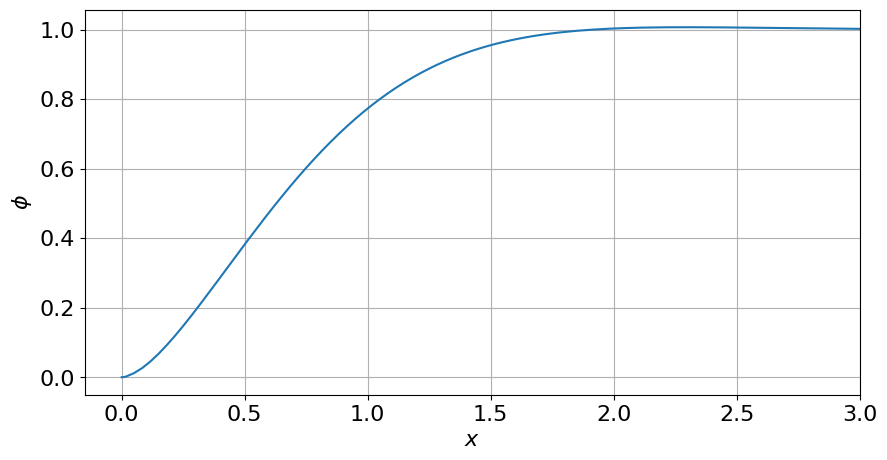
\includegraphics[width=0.81\textwidth]{../figures/result_volumes_cyl_bi.png}
\end{figure}
\vspace{-0.7cm}
\begin{center}
	Цилиндрический случай, $\alpha = 1$: особенность вида $r^2 (\ln r - 1)$
\end{center}
\end{frame}


\begin{frame}{Полученные результаты}
\vspace{-0.6cm}
\begin{figure}
	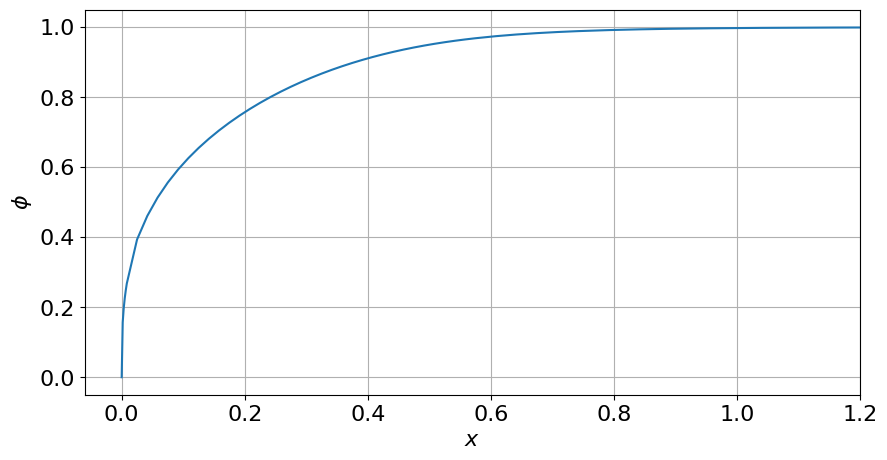
\includegraphics[width=0.81\textwidth]{../figures/result_volumes_sph_p.png}
\end{figure}
\vspace{-0.7cm}
\begin{center}
	Сферический случай, $\alpha = 0, \; \beta = 1$: особенность вида $r^{1/3}$
\end{center}
\end{frame}